% Here describe how did you come with your solution.
% In this section you need to describe:

% \begin{itemize}
%     \item What are you supposed to do, and why is it \emph{sound}.
%     \item What did you do, and what \emph{happened}
%     \item Provide a diagram of the software architecture of what you built. Remember there are various types of diagrams (e.g., contextual, structural, etc). Identify what the best diagram is for the purpose of your contribution.
% \end{itemize}

% All in all, this is the meat of the work, please show information about why what you did is important and how will you carry it forward.
% 1-2 pages is reasonable for this.

% arch.tex
% \section{System Architecture and Approach}
Our solution rests on two core components—a malicious test server and custom Scrapy spiders—glued together by a Flask orchestration UI.

\begin{itemize}
  \item \textbf{Malicious Flask Server:} Hosts endpoints for SQLi (`/sqli`), reflected XSS (`/xss_script`), and malware downloads (`/malware`), each intentionally lacking sanitization or content validation.
  \item \textbf{Scrapy Spiders:}
    \begin{itemize}
      \item \emph{SQLi Spider:} Submits FormRequests with tautologies and destructive payloads.
      \item \emph{XSS Spider:} Uses `scrapy-playwright` to render pages and override `window.alert()` via `add_init_script`.
      \item \emph{Malware Spider:} Follows download links and saves binaries without inspection.
    \end{itemize}
  \item \textbf{Flask Orchestration UI:} Provides “Trigger Crawl” buttons, in‐memory logging, and a live `/logs` dashboard (auto‐refresh).
\end{itemize}

\begin{figure*}[!t]
  \centering
  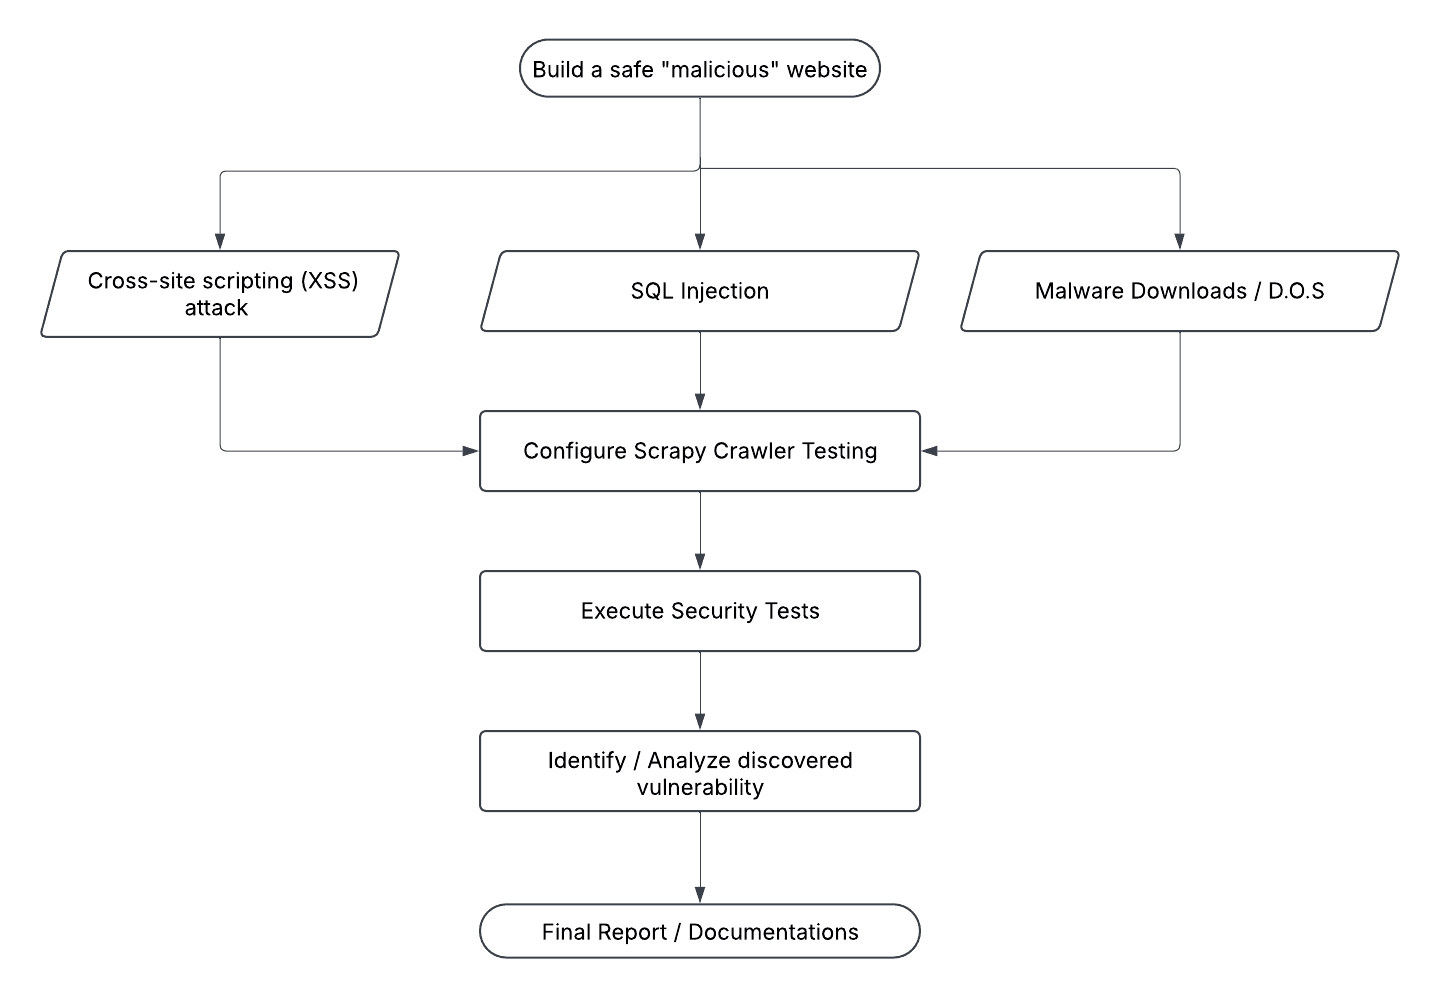
\includegraphics[width=\textwidth]{figures/blockarch.png}
  \caption{System architecture of ScrapyShield.}
  \label{fig:architecture}
\end{figure*}

\section{Project Design and Approach}

\subsection{i) System Overview}
To assess Scrapy’s vulnerability handling capabilities, we created a controlled sandbox environment composed of two main components: a malicious Flask-based web server and customized Scrapy spiders. The server hosted deliberately vulnerable endpoints simulating common attack vectors. Scrapy crawlers were adapted to interact with these endpoints, submitting inputs, parsing responses, and logging observed behavior. All testing was conducted in a closed environment without external network interaction, in adherence to ethical security testing practices.

\subsection{ii) Malicious Flask Server Design}
The Flask server contained routes representing different attack surfaces:
\begin{description}[leftmargin=1cm,style=nextline,itemsep=4pt]
  \item[\textbf{SQL Injection (\texttt{/sqli}):}]  
    A simple login form vulnerable to unsanitized SQL queries, allowing basic authentication-bypass attacks.
  \item[\textbf{Cross-Site Scripting (\texttt{/xss}, \texttt{/xss\_script}, \texttt{/xss\_img}, \texttt{/xss\_iframe}):}]  
    Multiple pages with reflective and stored XSS vulnerabilities, including injection via text fields and image attributes.
  \item[\textbf{Malware Downloads (\texttt{/malware}, \texttt{/disguised\_download}):}]  
    Pages offering files disguised as documents or installers, simulating drive-by download scenarios.
\end{description}
Each page was intentionally misconfigured to lack input validation, enabling a variety of simulated attacks.

\subsection{iii) Scrapy Spider Development}
Separate Scrapy spiders were developed for each attack type:
\begin{description}[leftmargin=1cm,style=nextline,itemsep=4pt]
  \item[\textbf{SQLi Spider:}]  
    Used \texttt{FormRequest} submissions to inject common SQLi payloads (e.g., \texttt{' OR 1=1 --}) into login forms and observed server responses.
  \item[\textbf{XSS Spider:}]  
    (Placeholder— to be completed by teammates)
  \item[\textbf{Malware Spider:}]  
    (Placeholder— to be completed by teammates)
\end{description}
The spiders were triggered asynchronously from the Flask web interface, allowing real-time attack launches without blocking the server’s functionality.

\subsection{iv) Logging and Monitoring Setup}
An in-memory logging system was integrated into the Flask server to capture attack attempts submitted to vulnerable forms. Logs included:
\begin{itemize}[topsep=2pt,itemsep=2pt]
  \item Payloads submitted  
  \item Timestamps  
  \item Response outcomes (e.g., success/failure messages)
\end{itemize}
A \texttt{/logs} endpoint displayed the recorded data through an auto-refreshing HTML dashboard, enabling live monitoring of crawler activities and attack success/failure rates. Trigger buttons were added to launch crawlers directly from the web interface, improving usability and rapid testing cycles.









